\documentclass{article}\usepackage[]{graphicx}\usepackage{xcolor}
%% maxwidth is the original width if it is less than linewidth
%% otherwise use linewidth (to make sure the graphics do not exceed the margin)
\makeatletter
\def\maxwidth{ %
  \ifdim\Gin@nat@width>\linewidth
    \linewidth
  \else
    \Gin@nat@width
  \fi
}
\makeatother

\definecolor{fgcolor}{rgb}{0.345, 0.345, 0.345}
\newcommand{\hlnum}[1]{\textcolor[rgb]{0.686,0.059,0.569}{#1}}%
\newcommand{\hlstr}[1]{\textcolor[rgb]{0.192,0.494,0.8}{#1}}%
\newcommand{\hlcom}[1]{\textcolor[rgb]{0.678,0.584,0.686}{\textit{#1}}}%
\newcommand{\hlopt}[1]{\textcolor[rgb]{0,0,0}{#1}}%
\newcommand{\hlstd}[1]{\textcolor[rgb]{0.345,0.345,0.345}{#1}}%
\newcommand{\hlkwa}[1]{\textcolor[rgb]{0.161,0.373,0.58}{\textbf{#1}}}%
\newcommand{\hlkwb}[1]{\textcolor[rgb]{0.69,0.353,0.396}{#1}}%
\newcommand{\hlkwc}[1]{\textcolor[rgb]{0.333,0.667,0.333}{#1}}%
\newcommand{\hlkwd}[1]{\textcolor[rgb]{0.737,0.353,0.396}{\textbf{#1}}}%

\usepackage{framed}
\makeatletter
\newenvironment{kframe}{%
 \def\at@end@of@kframe{}%
 \ifinner\ifhmode%
  \def\at@end@of@kframe{\end{minipage}}%
  \begin{minipage}{\columnwidth}%
 \fi\fi%
 \def\FrameCommand##1{\hskip\@totalleftmargin \hskip-\fboxsep
 \colorbox{shadecolor}{##1}\hskip-\fboxsep
     % There is no \\@totalrightmargin, so:
     \hskip-\linewidth \hskip-\@totalleftmargin \hskip\columnwidth}%
 \MakeFramed {\advance\hsize-\width
   \@totalleftmargin\z@ \linewidth\hsize
   \@setminipage}}%
 {\par\unskip\endMakeFramed%
 \at@end@of@kframe}
\makeatother

\definecolor{shadecolor}{rgb}{.97, .97, .97}
\definecolor{messagecolor}{rgb}{0, 0, 0}
\definecolor{warningcolor}{rgb}{1, 0, 1}
\definecolor{errorcolor}{rgb}{1, 0, 0}
\newenvironment{knitrout}{}{} % an empty environment to be redefined in TeX

\usepackage{alltt}
\IfFileExists{upquote.sty}{\usepackage{upquote}}{}
\begin{document}




\begin{knitrout}
\definecolor{shadecolor}{rgb}{0.969, 0.969, 0.969}\color{fgcolor}\begin{figure}
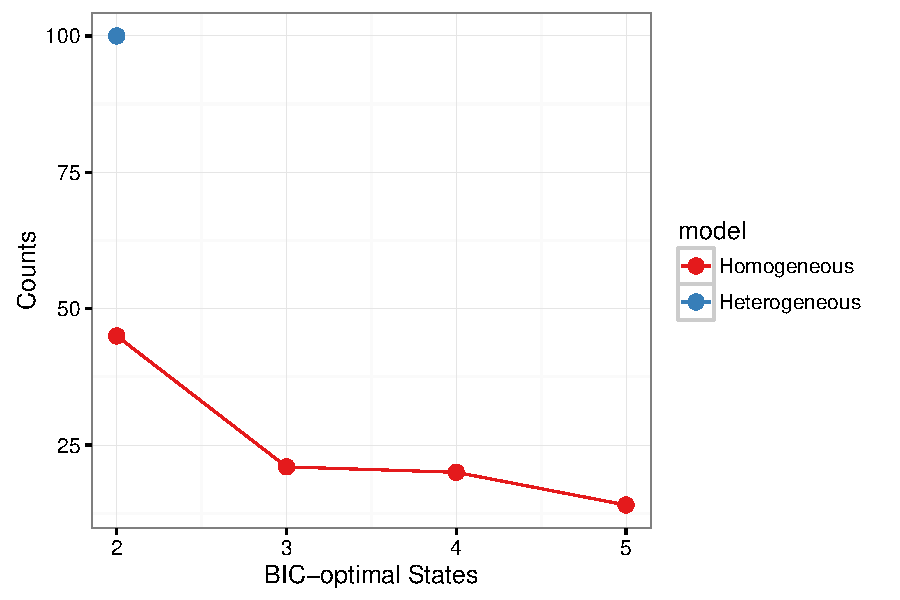
\includegraphics[width=\maxwidth]{figure/sim_results-1} \caption[BIC-optimal state frequency for 2-6 state HMMs with and without covariate transition on 100 two-state hidden Markov models with covariate transitioning simulations]{BIC-optimal state frequency for 2-6 state HMMs with and without covariate transition on 100 two-state hidden Markov models with covariate transitioning simulations.}\label{fig:sim_results}
\end{figure}


\end{knitrout}


\clearpage


\begin{knitrout}
\definecolor{shadecolor}{rgb}{0.969, 0.969, 0.969}\color{fgcolor}\begin{figure}
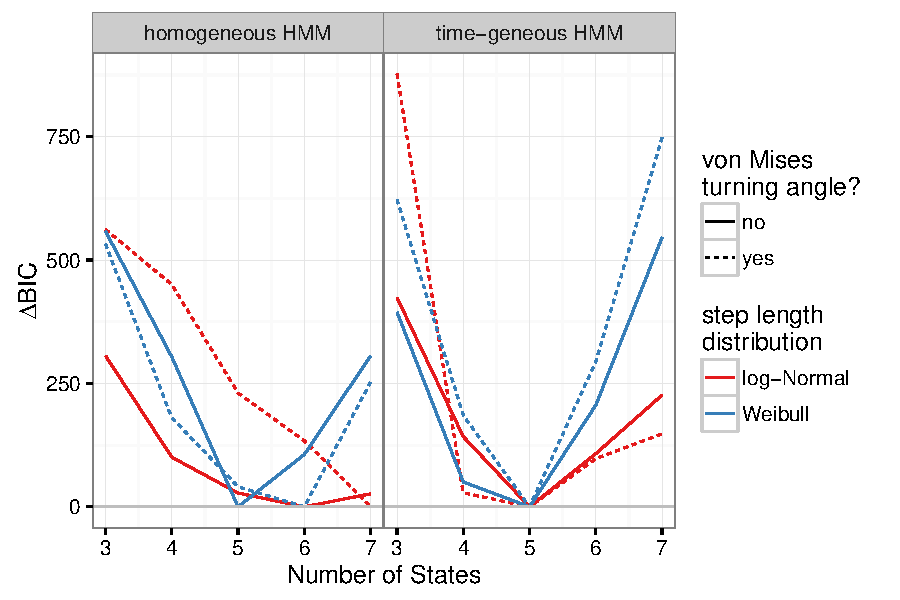
\includegraphics[width=\maxwidth]{figure/BICred_plot-1} \caption[Adjusted Bayesian information criterion values for 3-7 state HMMs with different step-length distributions, with and without temporal transitions and turning angles]{Adjusted Bayesian information criterion values for 3-7 state HMMs with different step-length distributions, with and without temporal transitions and turning angles.}\label{fig:BICred_plot}
\end{figure}


\end{knitrout}


\clearpage

\begin{knitrout}
\definecolor{shadecolor}{rgb}{0.969, 0.969, 0.969}\color{fgcolor}\begin{figure}
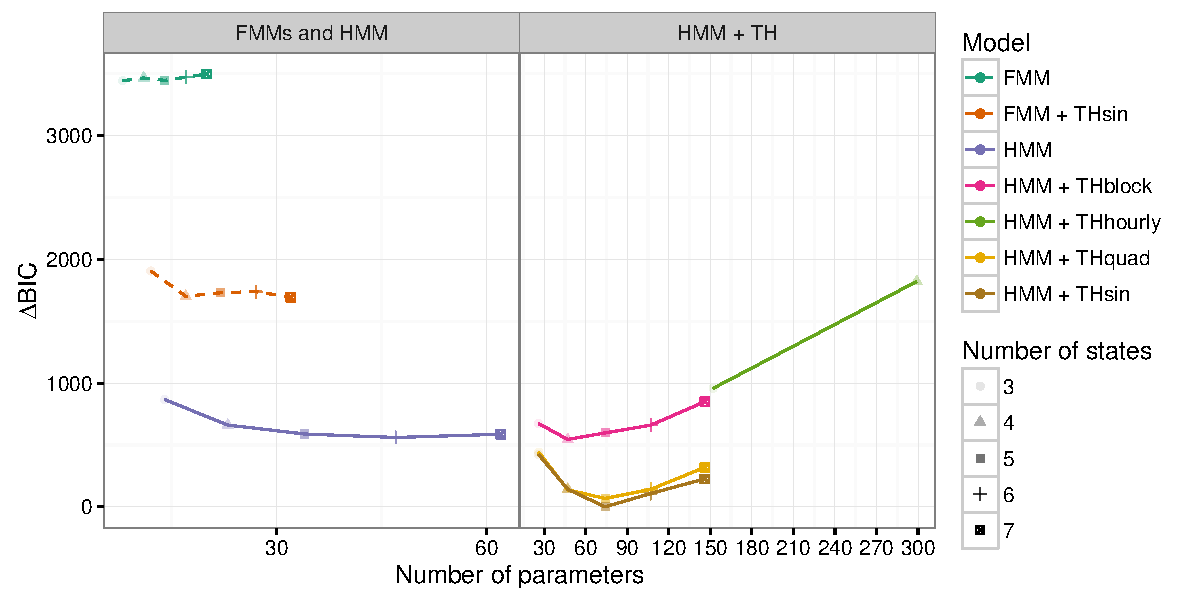
\includegraphics[width=\maxwidth]{figure/adj_BIC_comparisons-1} \caption[Adjusted BIC by number of free parameters for HMM model types]{Adjusted BIC by number of free parameters for HMM model types. The left panel shows FMM, temporally heterogeneous FMM with a sinusoidal prior and HMM. The right panel shows HMMs with different temporal transitions.}\label{fig:adj_BIC_comparisons}
\end{figure}


\end{knitrout}

\clearpage

\begin{knitrout}
\definecolor{shadecolor}{rgb}{0.969, 0.969, 0.969}\color{fgcolor}\begin{figure}
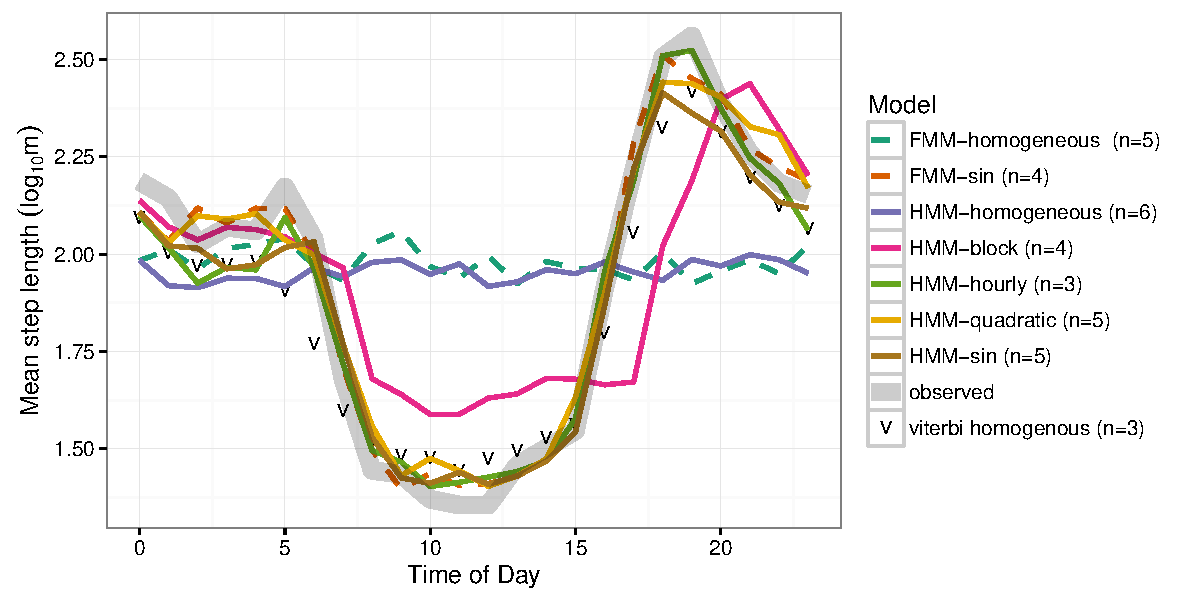
\includegraphics[width=\maxwidth]{figure/avg_step_length_by_time-1} \caption[Average step length by time of day observed (gray highlight), three-state HMM Viterbi predictions (V points), and all transitions type HMMs predictions (out of sample) with their respective BIC-optimal states]{Average step length by time of day observed (gray highlight), three-state HMM Viterbi predictions (V points), and all transitions type HMMs predictions (out of sample) with their respective BIC-optimal states.}\label{fig:avg_step_length_by_time}
\end{figure}


\end{knitrout}

\clearpage

\begin{knitrout}
\definecolor{shadecolor}{rgb}{0.969, 0.969, 0.969}\color{fgcolor}\begin{figure}
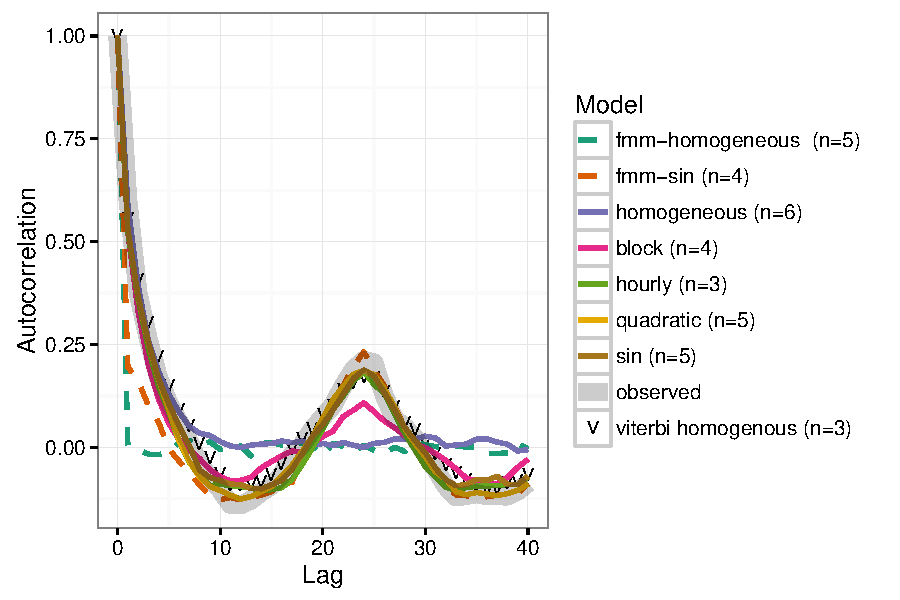
\includegraphics[width=\maxwidth]{figure/acf_plot-1} \caption[Autocorrelation of observed (gray highlight), three-state HMM Viterbi predictions (V points), and all transitions type HMMs predictions (out of sample) with their respective BIC-optimal states ]{Autocorrelation of observed (gray highlight), three-state HMM Viterbi predictions (V points), and all transitions type HMMs predictions (out of sample) with their respective BIC-optimal states }\label{fig:acf_plot}
\end{figure}


\end{knitrout}

\clearpage

\begin{knitrout}
\definecolor{shadecolor}{rgb}{0.969, 0.969, 0.969}\color{fgcolor}\begin{figure}
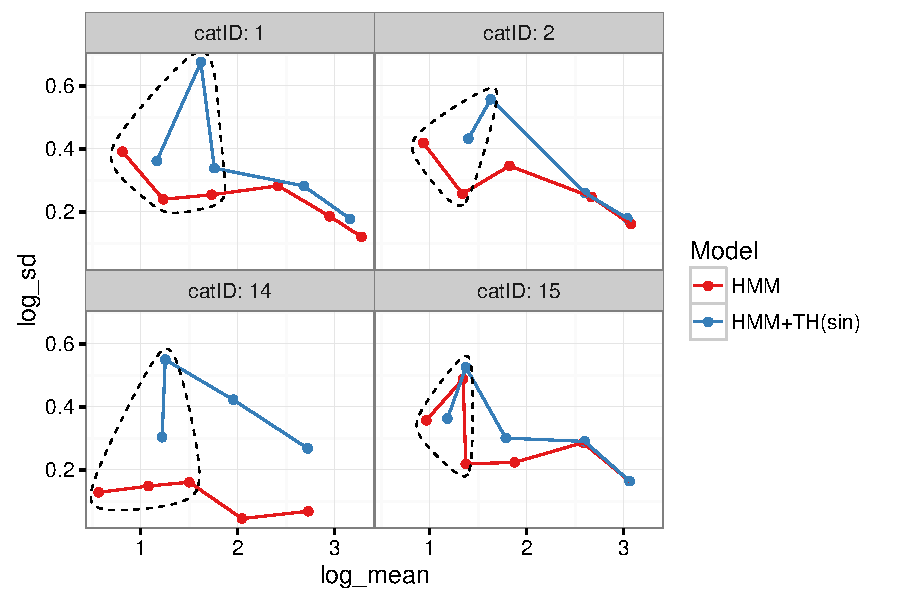
\includegraphics[width=\maxwidth]{figure/r_msdlist-1} \caption[State identification plot with log mean and standard deviation of BIC-optimal HMM and HMM with sinusoidal transition]{State identification plot with log mean and standard deviation of BIC-optimal HMM and HMM with sinusoidal transition.}\label{fig:r msdlist}
\end{figure}


\end{knitrout}

\clearpage

\section{Additional files}


\begin{knitrout}
\definecolor{shadecolor}{rgb}{0.969, 0.969, 0.969}\color{fgcolor}
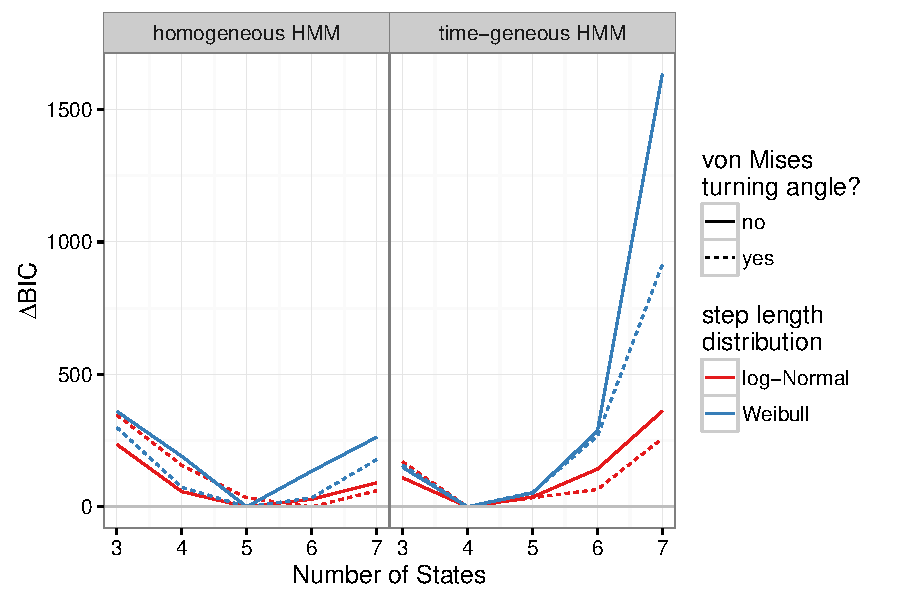
\includegraphics[width=\maxwidth]{figure/BICred_plot2-1} 

\end{knitrout}


\clearpage


\begin{knitrout}
\definecolor{shadecolor}{rgb}{0.969, 0.969, 0.969}\color{fgcolor}
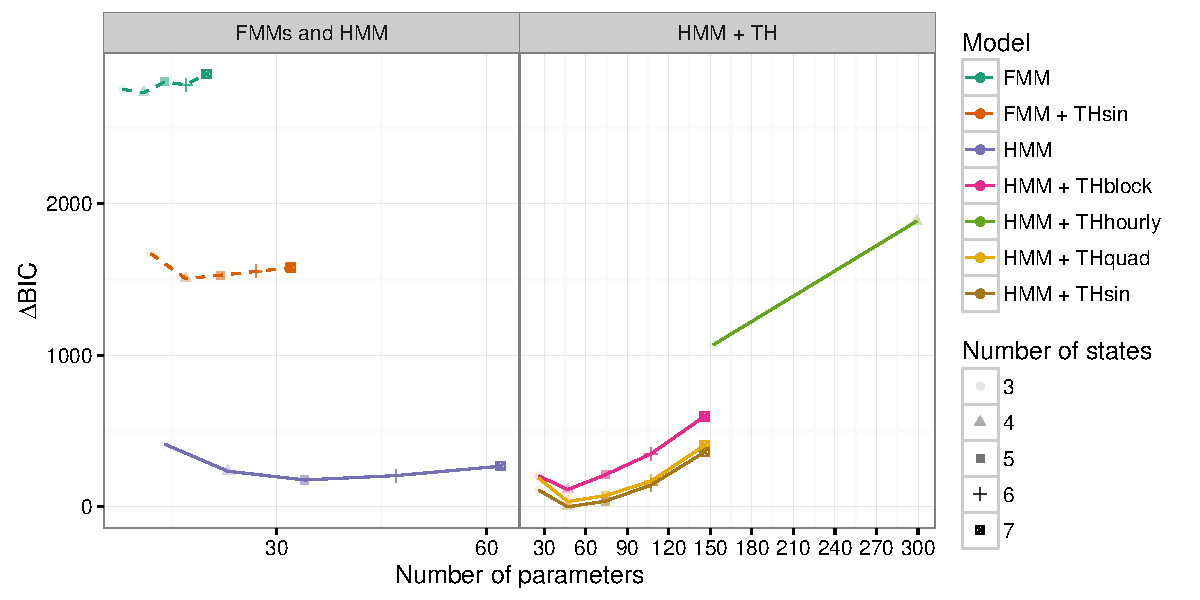
\includegraphics[width=\maxwidth]{figure/adj_BIC_comparisons2-1} 

\end{knitrout}

\clearpage

\begin{knitrout}
\definecolor{shadecolor}{rgb}{0.969, 0.969, 0.969}\color{fgcolor}
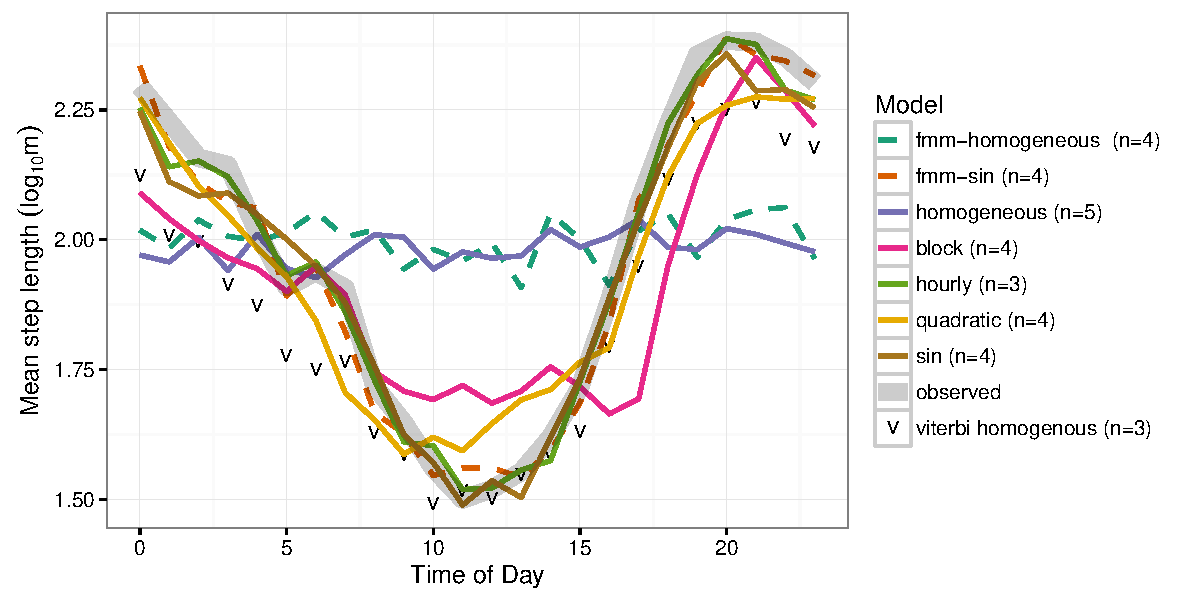
\includegraphics[width=\maxwidth]{figure/avg_step_length_by_time2-1} 

\end{knitrout}

\clearpage

\begin{knitrout}
\definecolor{shadecolor}{rgb}{0.969, 0.969, 0.969}\color{fgcolor}
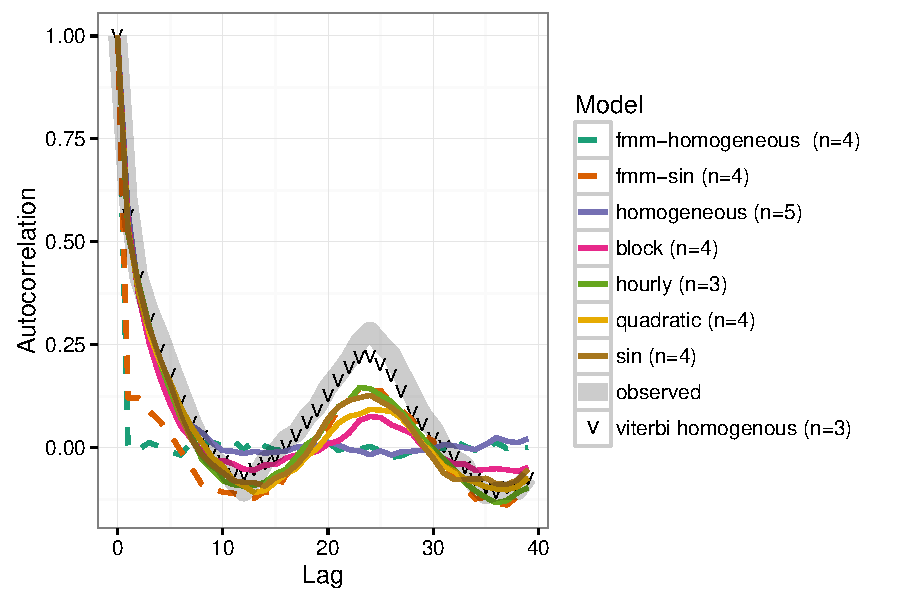
\includegraphics[width=\maxwidth]{figure/acf_plot2-1} 

\end{knitrout}


\clearpage
%cat14

\begin{knitrout}
\definecolor{shadecolor}{rgb}{0.969, 0.969, 0.969}\color{fgcolor}
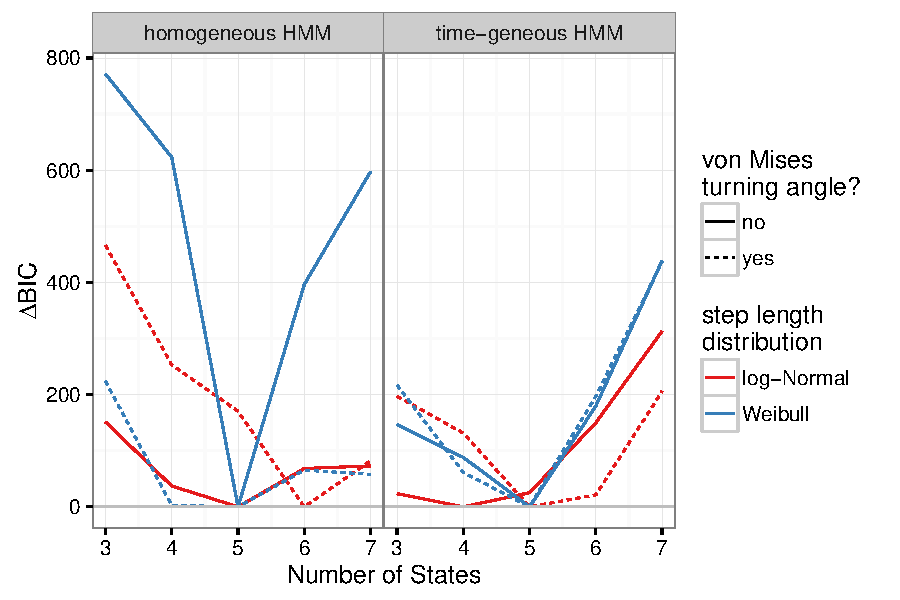
\includegraphics[width=\maxwidth]{figure/BICred_plot14-1} 

\end{knitrout}


\clearpage

\begin{knitrout}
\definecolor{shadecolor}{rgb}{0.969, 0.969, 0.969}\color{fgcolor}
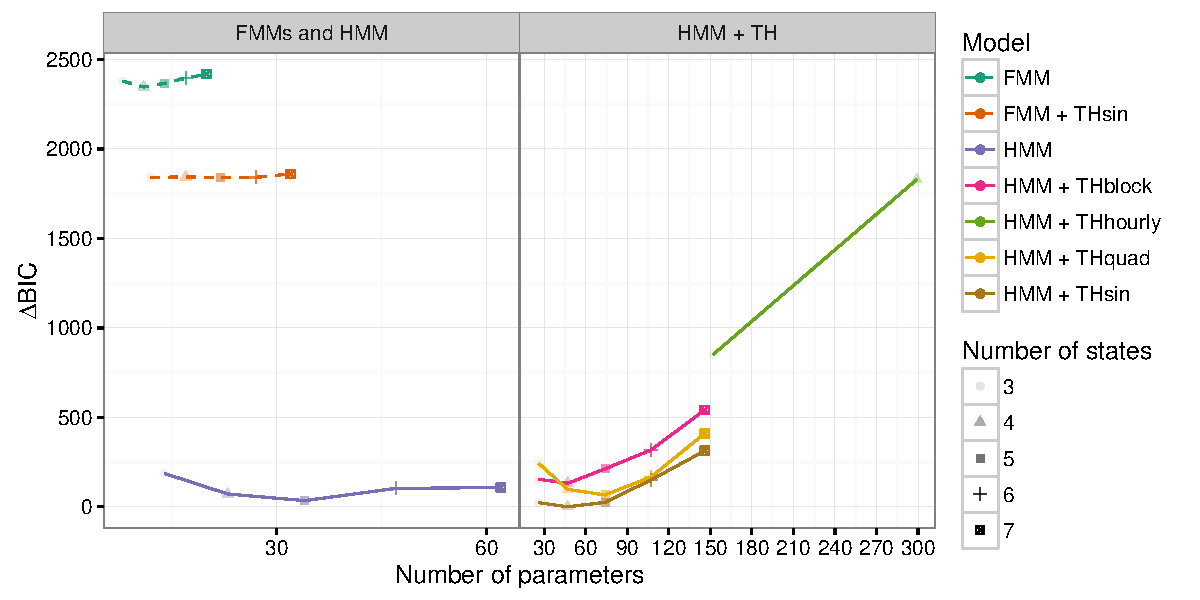
\includegraphics[width=\maxwidth]{figure/adj_BIC_comparisons14-1} 

\end{knitrout}

\clearpage

\begin{knitrout}
\definecolor{shadecolor}{rgb}{0.969, 0.969, 0.969}\color{fgcolor}
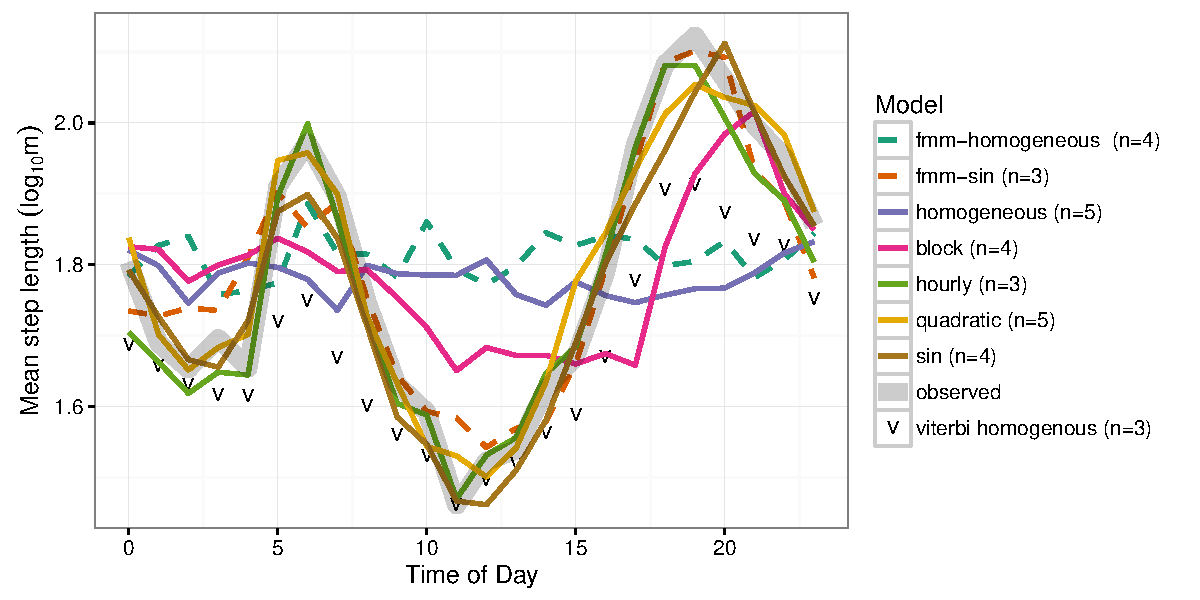
\includegraphics[width=\maxwidth]{figure/avg_step_length_by_time14-1} 

\end{knitrout}

\clearpage

\begin{knitrout}
\definecolor{shadecolor}{rgb}{0.969, 0.969, 0.969}\color{fgcolor}
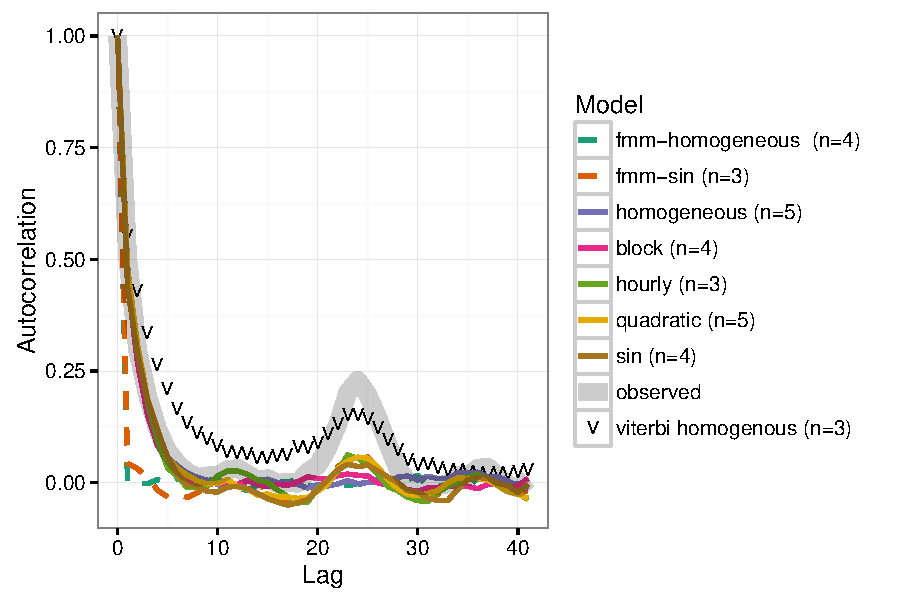
\includegraphics[width=\maxwidth]{figure/acf_plot14-1} 

\end{knitrout}

\clearpage
%cat15

\begin{knitrout}
\definecolor{shadecolor}{rgb}{0.969, 0.969, 0.969}\color{fgcolor}
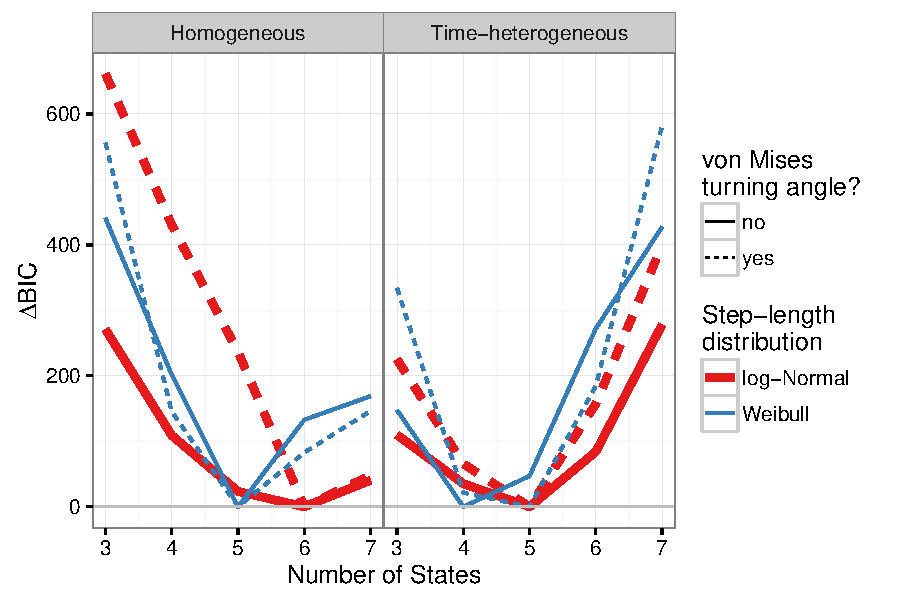
\includegraphics[width=\maxwidth]{figure/BICred_plot15-1} 

\end{knitrout}


\clearpage

\begin{knitrout}
\definecolor{shadecolor}{rgb}{0.969, 0.969, 0.969}\color{fgcolor}
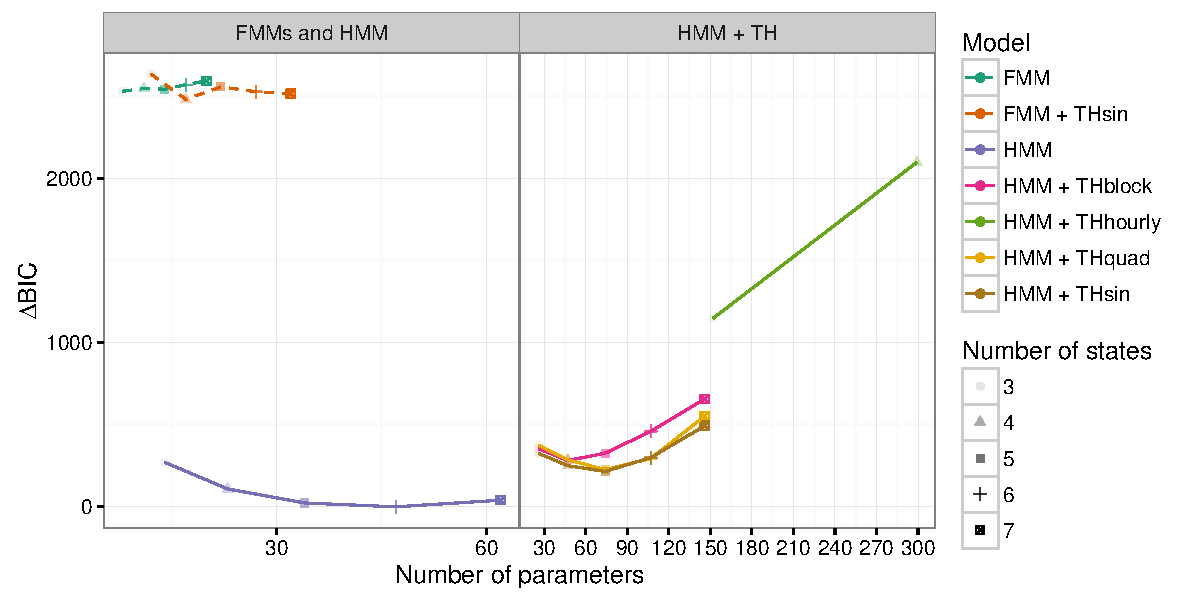
\includegraphics[width=\maxwidth]{figure/adj_BIC_comparisons15-1} 

\end{knitrout}

\clearpage

\begin{knitrout}
\definecolor{shadecolor}{rgb}{0.969, 0.969, 0.969}\color{fgcolor}
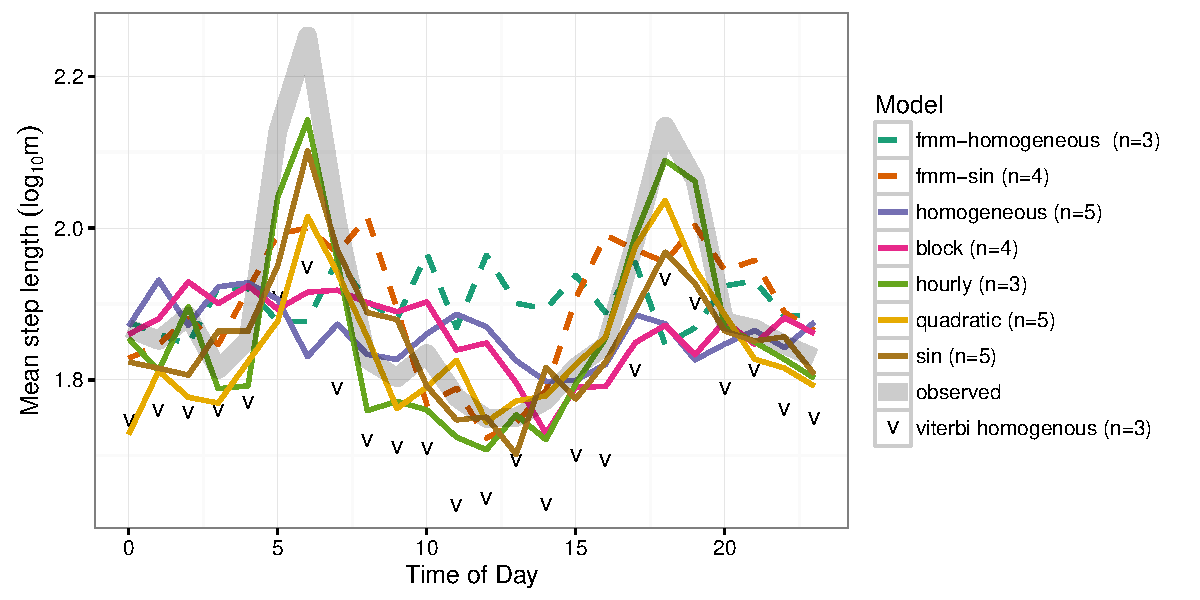
\includegraphics[width=\maxwidth]{figure/avg_step_length_by_time15-1} 

\end{knitrout}

\clearpage

\begin{knitrout}
\definecolor{shadecolor}{rgb}{0.969, 0.969, 0.969}\color{fgcolor}
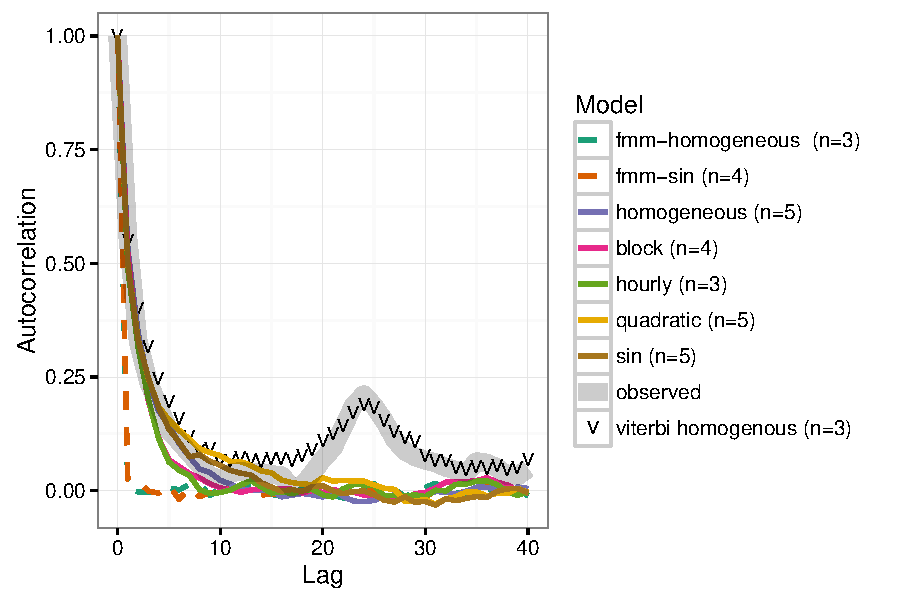
\includegraphics[width=\maxwidth]{figure/acf_plot15-1} 

\end{knitrout}

\end{document}
